% GNUPLOT: LaTeX picture with Postscript
\begingroup
  \makeatletter
  \providecommand\color[2][]{%
    \GenericError{(gnuplot) \space\space\space\@spaces}{%
      Package color not loaded in conjunction with
      terminal option `colourtext'%
    }{See the gnuplot documentation for explanation.%
    }{Either use 'blacktext' in gnuplot or load the package
      color.sty in LaTeX.}%
    \renewcommand\color[2][]{}%
  }%
  \providecommand\includegraphics[2][]{%
    \GenericError{(gnuplot) \space\space\space\@spaces}{%
      Package graphicx or graphics not loaded%
    }{See the gnuplot documentation for explanation.%
    }{The gnuplot epslatex terminal needs graphicx.sty or graphics.sty.}%
    \renewcommand\includegraphics[2][]{}%
  }%
  \providecommand\rotatebox[2]{#2}%
  \@ifundefined{ifGPcolor}{%
    \newif\ifGPcolor
    \GPcolorfalse
  }{}%
  \@ifundefined{ifGPblacktext}{%
    \newif\ifGPblacktext
    \GPblacktexttrue
  }{}%
  % define a \g@addto@macro without @ in the name:
  \let\gplgaddtomacro\g@addto@macro
  % define empty templates for all commands taking text:
  \gdef\gplfronttext{}%
  \gdef\gplfronttext{}%
  \makeatother
  \ifGPblacktext
    % no textcolor at all
    \def\colorrgb#1{}%
    \def\colorgray#1{}%
  \else
    % gray or color?
    \ifGPcolor
      \def\colorrgb#1{\color[rgb]{#1}}%
      \def\colorgray#1{\color[gray]{#1}}%
      \expandafter\def\csname LTw\endcsname{\color{white}}%
      \expandafter\def\csname LTb\endcsname{\color{black}}%
      \expandafter\def\csname LTa\endcsname{\color{black}}%
      \expandafter\def\csname LT0\endcsname{\color[rgb]{1,0,0}}%
      \expandafter\def\csname LT1\endcsname{\color[rgb]{0,1,0}}%
      \expandafter\def\csname LT2\endcsname{\color[rgb]{0,0,1}}%
      \expandafter\def\csname LT3\endcsname{\color[rgb]{1,0,1}}%
      \expandafter\def\csname LT4\endcsname{\color[rgb]{0,1,1}}%
      \expandafter\def\csname LT5\endcsname{\color[rgb]{1,1,0}}%
      \expandafter\def\csname LT6\endcsname{\color[rgb]{0,0,0}}%
      \expandafter\def\csname LT7\endcsname{\color[rgb]{1,0.3,0}}%
      \expandafter\def\csname LT8\endcsname{\color[rgb]{0.5,0.5,0.5}}%
    \else
      % gray
      \def\colorrgb#1{\color{black}}%
      \def\colorgray#1{\color[gray]{#1}}%
      \expandafter\def\csname LTw\endcsname{\color{white}}%
      \expandafter\def\csname LTb\endcsname{\color{black}}%
      \expandafter\def\csname LTa\endcsname{\color{black}}%
      \expandafter\def\csname LT0\endcsname{\color{black}}%
      \expandafter\def\csname LT1\endcsname{\color{black}}%
      \expandafter\def\csname LT2\endcsname{\color{black}}%
      \expandafter\def\csname LT3\endcsname{\color{black}}%
      \expandafter\def\csname LT4\endcsname{\color{black}}%
      \expandafter\def\csname LT5\endcsname{\color{black}}%
      \expandafter\def\csname LT6\endcsname{\color{black}}%
      \expandafter\def\csname LT7\endcsname{\color{black}}%
      \expandafter\def\csname LT8\endcsname{\color{black}}%
    \fi
  \fi
    \setlength{\unitlength}{0.0500bp}%
    \ifx\gptboxheight\undefined%
      \newlength{\gptboxheight}%
      \newlength{\gptboxwidth}%
      \newsavebox{\gptboxtext}%
    \fi%
    \setlength{\fboxrule}{0.5pt}%
    \setlength{\fboxsep}{1pt}%
\begin{picture}(5000.00,5500.00)%
    \gplgaddtomacro\gplfronttext{%
      \colorrgb{0.15,0.15,0.15}%
      \put(368,3217){\makebox(0,0)[r]{\strut{}$0$}}%
      \colorrgb{0.15,0.15,0.15}%
      \put(368,3505){\makebox(0,0)[r]{\strut{}$c_0$}}%
      \colorrgb{0.15,0.15,0.15}%
      \put(368,3794){\makebox(0,0)[r]{\strut{}$400$}}%
      \colorrgb{0.15,0.15,0.15}%
      \put(368,4372){\makebox(0,0)[r]{\strut{}$800$}}%
      \colorrgb{0.15,0.15,0.15}%
      \put(368,4949){\makebox(0,0)[r]{\strut{}$1200$}}%
      \colorrgb{0.15,0.15,0.15}%
      \put(500,2997){\makebox(0,0){\strut{}$0$}}%
      \colorrgb{0.15,0.15,0.15}%
      \put(1100,2997){\makebox(0,0){\strut{}$\delta_0$}}%
      \colorrgb{0.15,0.15,0.15}%
      \put(1833,2997){\makebox(0,0){\strut{}$1.5$}}%
      \colorrgb{0.15,0.15,0.15}%
      \put(3166,2997){\makebox(0,0){\strut{}$3$}}%
      \colorrgb{0.15,0.15,0.15}%
      \put(4499,2997){\makebox(0,0){\strut{}$4.5$}}%
    }%
    \gplgaddtomacro\gplfronttext{%
      \colorrgb{0.15,0.15,0.15}%
      \put(-402,4083){\rotatebox{90}{\makebox(0,0){\strut{}CAER [m]}}}%
      \colorrgb{0.15,0.15,0.15}%
      \put(2499,2667){\makebox(0,0){\strut{}pose estimate error [(m$^2$ + rad$^2$)$^{1/2}$]}}%
      \put(1013,3330){\makebox(0,0){$\mathcal{V}$}}%
      \put(2600,4000){\makebox(0,0){\color{white}$\hat{\bm{p}} \in \mathcal{H} \backslash \mathcal{V} : \|\bm{p}-\hat{\bm{p}}\|_2 \geq \delta_0$}}%
    }%
    \gplgaddtomacro\gplfronttext{%
      \colorrgb{0.15,0.15,0.15}%
      \put(368,550){\makebox(0,0)[r]{\strut{}$0$}}%
      \colorrgb{0.15,0.15,0.15}%
      \put(368,810){\makebox(0,0)[r]{\strut{}$\delta_0$}}%
      \colorrgb{0.15,0.15,0.15}%
      \put(368,1127){\makebox(0,0)[r]{\strut{}$1.5$}}%
      \colorrgb{0.15,0.15,0.15}%
      \put(368,1705){\makebox(0,0)[r]{\strut{}$3.0$}}%
      \colorrgb{0.15,0.15,0.15}%
      \put(368,2282){\makebox(0,0)[r]{\strut{}$4.5$}}%
      \colorrgb{0.15,0.15,0.15}%
      \put(1300,330){\makebox(0,0){\strut{}$10^1$}}%
      \colorrgb{0.15,0.15,0.15}%
      \put(2100,330){\makebox(0,0){\strut{}$10^2$}}%
      \colorrgb{0.15,0.15,0.15}%
      \put(2899,330){\makebox(0,0){\strut{}$10^3$}}%
      \colorrgb{0.15,0.15,0.15}%
      \put(3699,330){\makebox(0,0){\strut{}$10^4$}}%
      \colorrgb{0.15,0.15,0.15}%
      \put(4499,330){\makebox(0,0){\strut{}$10^5$}}%
    }%
    \gplgaddtomacro\gplfronttext{%
      \colorrgb{0.15,0.15,0.15}%
      \put(-1194,1416){\rotatebox{90}{\makebox(0,0){\strut{}pose estimate error [(m$^2$ + rad$^2$)$^{1/2}$]}}}%
      \colorrgb{0.15,0.15,0.15}%
      \put(2499,0){\makebox(0,0){\strut{}position in ascending CAER hierarchy}}%
    }%
    \put(0,0){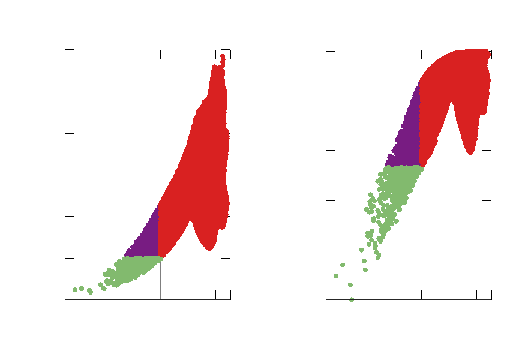
\includegraphics{./figures/h_fig}}%
    \gplfronttext
  \end{picture}%
\endgroup
